% we should list the event log definition and petri net definition
% also the process tree definition
% For definitions, we capitalize only the first character, others we use camel methods. 
This chapter introduces the most important ground concepts and notations that are used in this thesis. 
\section{Event Log}
% introduce of event and trace , later event log historical business process execution data in information systems
Business process in organizations is reflected by its execution of a set of activities. The historical execution data is usually in a form of event logs in information systems and can be used by Process Mining to analyze the business execution. To specify the event log, we begin with formalizing the various notations\cite{van2016data} .
\begin{definition}[Event]
	An event corresponds to an activity in business execution and can be marked by $e$. An event is characterized by attributes, like a timestamp, name, and associated costs, etc. The finite set of events in the process is written as $\mathcal{E}$.
\end{definition}
\begin{definition}[Trace]
A trace is a finite sequence of events $\sigma \in \mathcal{E}^*$ with conditions that \emph{(i)} each event can not appear twice in a trace, $ \forall i,j, 1 \leq i,j \leq \vert \sigma \vert, if \ i \neq j, then\ \sigma (i) \neq \sigma (j) $.  \emph{(ii)} one event can only appear in one trace, $ \forall e \in \sigma, if\ e \in \sigma\prime, then\ \sigma = \sigma\prime $. 
A trace also has a set of attributes, which describes the trace characters, like the identifier, the trace cost.
\end{definition}
\begin{definition}[Event log]
An event log $L$ is a set of traces. If an event log contains timestamps, then the ordering in a trace should respect these timestamps. 
\end{definition}
\section{Process Models}
After gathering the event log from information systems, process mining can discover a process model based on the event log, aims to improve understanding and insights on the business process. Multiple process modeling languages are applied in process mining in the last years, such as Petri net, BPMN models, etc. Among multiple models which are proposed to describe business processes, Petri net has been best studied thoroughly to allow for the modeling of concurrency of activities and is one of the main models in process mining. Process tree is based on a tree structure to organize the event relation and simple to understand in comparison with other models. In this thesis, those two models are used to represent process models.
\subsection{Petri Net}
Petri nets are bipartite graph to describe concurrent systems. Activities from event log correspond to observable transitions in Petri net. Places in Petri net connect the transitions to express execution rules of activities. Except the observable transitions, there are silent transitions which are not visible and used to build certain model structures. 
\begin{definition}[Silent transition]
	A silent transition, usually denoted by $\epsilon$, is an internal transition that is non-observable from the outside but builds certain structures in Petri net. In dynamic view, it can be used to express the different states of the Petri net. 
\end{definition}
The observable transitions with silent transition ground a basic element set for the static structure of Petri net. To describe the dynamic behaviors of Petri net, the concept called \emph{token} is introduced. It is a mark in the place to enable execution of the following transition. If all the input places for a transition hold a token, the transition becomes enabled. In other words, the corresponding activity can be triggered. After this execution, the token in the input places are consumed and new tokens are generated in the output places. Initially, only the start place contains a token. 
% Begin to introduce the event log 
\begin{definition}[Petri net]
	A Petri net N is composed of a finite set of places P, transitions T, and a set of directed arcs $F \subseteq (P \times T) \cup (T \times P)$, which can be written as $N=(P,T,F)$. A marked Petri net is (P,T,F,M) where M the marking of the net. A marking of a net N is a multi-set over P, $M \in \mathbb{P} $ and used to express the dynamic state of the Petri net.
\end{definition}

An example is shown in Figure \ref{fig:pn-seq-2}. It has transitions $T=\{A,B,C,D,E\}$ and four places with the initial marking in the place before $T=\{A,B\}$. 
\begin{figure}[!h]
	\centering
	\begin{subfigure}[b]{0.45\textwidth}
		\centering
		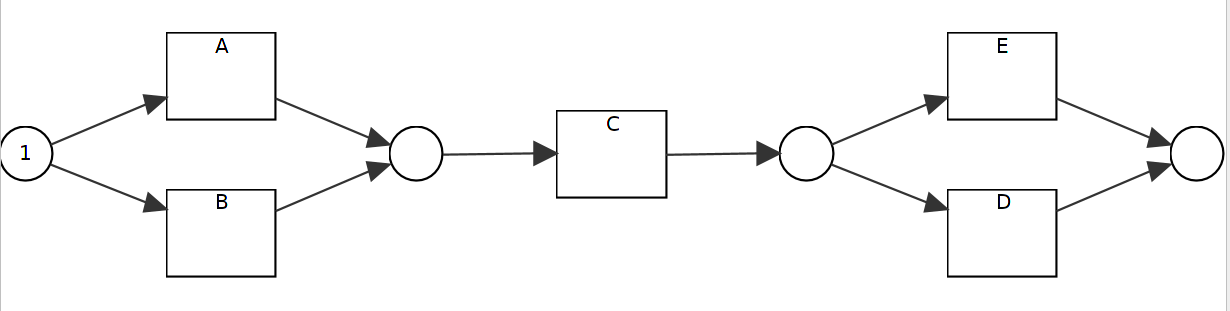
\includegraphics[width=\linewidth]{figures/preliminary/PN06_Seq_2_xor_notnested.png}
		\caption{A Simple Petri net}
		\label{fig:pn-seq-2}
	\end{subfigure}%
	\quad
	\begin{subfigure}[b]{0.45\textwidth}
		\centering
		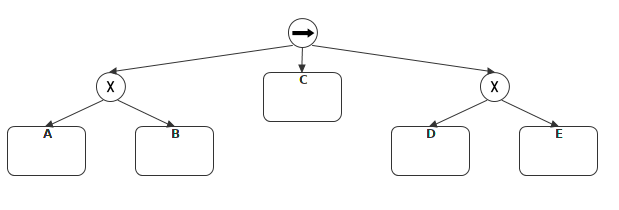
\includegraphics[width=\linewidth]{figures/preliminary/PT06_Seq_2_xor_notnested.png}
		\caption{A process tree corresponding to Fig \ref{fig:pn-seq-2}}
		\label{fig:pt-seq-2}
	\end{subfigure}%
\end{figure}
%% Here add the definition for soundness

The correctness of business process models is necessary to perform the business on an enterprise level. Soundness defines a minimum correctness criterion that a process model should satisfy\cite{van2006structural}. In the following, we give the definition of soundness for Petri net.
\begin{definition}[Soundness]
	A Petri net is sound if and only if it satisfies the following conditions.
	\begin{itemize}
		\itemsep0em 
		\item safeness. Places cannot hold multiple tokens at the same time.
		\item proper completion. If the sink place is marked, all other places are empty.
		\item option to complete. It is always possible to reach the final marking just for the sink place.
		\item no dead part. For any transition there is a path from source to sink place through it. 
	\end{itemize}
\end{definition}

\subsection{Process Tree}
Process tree is block-structured and sound by construction, while Petri nets, BPMN models possibly suffer from deadlocks, other anomalies\cite{van2016data}. Here we give the definition of process tree.
\begin{definition}[Process Tree]
Let $ A \subseteq \mathbb{A} $ be a finite set of activities with silent transition $\tau \in \mathbb{A}$, $\bigoplus \subseteq \{\rightarrow, \times, \land, \circlearrowright\}$ be the set of process tree operators. 
\begin{itemize}
\item $Q=a$ is a process tree with $a\in A$, and 
\item $Q= \oplus (Q_1 , Q_2 ,.. Q_n)$ is a process tree with $\oplus \in \bigoplus$, and $Q_i$ is a process tree, $i\in{1,2,..,n}, n\in \mathbb{N}$. 
\end{itemize}
\end{definition}

Process tree operators represents different block relation of each subtree. Their semantics are standardized from \cite{vanderAalst:2016:PMD:2948762, Buijs2012OnTR} and explained with use of Petri net in Figure \ref{fig:pn_pt_correspondings}\cite{Buijs2012OnTR}.
\begin{figure}[!h]
	\centering
	\begin{subfigure}[b]{0.45\textwidth}
		\centering
		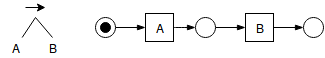
\includegraphics[width=\linewidth]{figures/preliminary/PT_PN_corresponding_01_seq_PN.png}
		\caption{Sequence}
		\label{fig:pt_pn_seq}
	\end{subfigure}%
	\quad
	\begin{subfigure}[b]{0.45\textwidth}
		\centering
		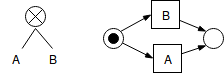
\includegraphics[width=\linewidth]{figures/preliminary/PT_PN_corresponding_02_xor_PN.png}
		\caption{Exclusive choice}
		\label{fig:pt_pn_xor}
	\end{subfigure}%
	\\ %this makes much difference
	\begin{subfigure}[b]{0.45\textwidth}
		\centering
		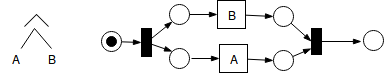
\includegraphics[width=\linewidth]{figures/preliminary/PT_PN_corresponding_03_and_PN.png}
		\caption{ Parallelism }
		\label{fig:pt_pn_and}
	\end{subfigure}%
	\quad
	\begin{subfigure}[b]{0.45\textwidth}
		\centering
		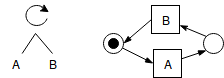
\includegraphics[width=\linewidth]{figures/preliminary/PT_PN_corresponding_04_loop_PN.png}
		\caption{Loop}
		\label{fig:pt_pn_loop}
	\end{subfigure}%
	\caption{Semantics of process tree operators w.r.t. Petri net}
	\label{fig:pn_pt_correspondings}
\end{figure}
\begin{definition}[Operator Semantics] 
	The semantics of operators $\bigoplus \subseteq \{\rightarrow, \times, \land, \circlearrowright \}$ are,
	\begin{itemize}
		\item if $Q= \rightarrow(Q_1 , Q_2 ,.. Q_n)$, the subtrees have sequential relation and are executed in order of $Q_1,Q_2,..Q_n$
		\item if $Q= \times(Q_1 , Q_2 ,.. Q_n)$,  the subtrees have exclusive choice relation and only one subtree of $Q_1,Q_2,..Q_n$   can be executed.
		\item if $Q= \land (Q_1 , Q_2 ,.. Q_n)$,  the subtrees have parallel relation and $Q_1,Q_2,..Q_n$ they can be executed in parallel.
		\item if $Q= \circlearrowright(Q_1 , Q_2 ,.. Q_n)$,  the subtrees have loop relation and $Q_1,Q_2,..Q_n \; with\; n\geq2$, $Q_1$ is the do-part and is executed at least once, $Q_2,..Q_n$ are redo part and have exclusive relation.
	\end{itemize}
\end{definition}
According to the corresponding semantic relations,  a process tree can be easily transformed into Petri net. In Figure \ref{fig:pt-seq-2}, it is the process model in process tree which describes the same process as in Figure \ref{fig:pn-seq-2}. 
%% here to describe the inductive miner 
\section{Inductive Miner}
To discover a process model from an event log, we choose one of the leading process discovery approaches -- Inductive Miner, because it guarantees the construction of a sound model, and is flexible and scalable to event log data. Its steps are listed bellow. 
\subsection{Construct a directly-follows graph}
A the start, the event log $L$ is scanned to extract the directly follows relation of events. The directly-follows relation is like the one in $\alpha$-algorithm \cite{van2004workflow, leemans2013discovering}, but the frequency information is stored for each relation. Later, those relations are combined together to build a directly-follows graph with frequency. According to \cite{van2016data, leemans2013discovering}, a directly-follows graph is defined bellow.
\begin{definition}[Directly-follows Graph]
 The directly-follows relation $a > b$ is satisfied iff there is a trace $\sigma\ where, \sigma(i)=a \ and \ \sigma(i+1)=b$.
 A directly-follows graph of an event log $L$ is $G(L) = (A, F, A_{start}, A_{end}) $ where $A$ is the set of activities in L, $F={(a,b) \in A \times A | a >_L b} $ is the directly-follows relation, $A_{start}, A_{end}$ are the set of start and end activities respectively.
\end{definition}
The frequency information of the directly-follows relation is called cardinality and defined below.
\begin{definition}[Cardinality in a directly-follows graph]
Given a directly-follows graph G(L) derived from an event log L, the cardinality of each directly-follows relation in G(L) is :  
	\begin{itemize}
		\item $Cardinality(E(A,B))$ is the frequency of traces with $\langle ...,A,B,... \rangle$. 
		\item Start node A cardinality $Cardinality(Start(A))$ is the frequency of traces with begin node A.
		\item End node B cardinality $Cardinality(End(A))$ is the frequency of traces with end node B.
	\end{itemize}	
\end{definition}
\subsection{Split Log Into Sublogs}
Based on the directly-follows graph, it finds the most prominent cut which is applied afterwards to split the event log into smaller sublogs. Cuts compose of \emph{exclusive-choice cut, sequence cut, parallel cut and redo-loop cut} which correspond to the process tree operators $ \{\rightarrow, \times, \land, \circlearrowright \}$. They are selected in the following order. A maximal exclusive-choice cut is firstly tried to split the directly-follows graph; if it is not available, then a maximal sequence cut, a  maximal parallel cut and a redo-loop cut are applied in sequence. Sublogs are created due to this available operator. Meanwhile, this operator is used to build the process tree. 

The same procedure is applied again on the sublogs until single activities. What's more, this process tree can be converted into Petri net for further analysis.

\iffalse
I'd like to put this part into the evaluation section.
\section{Model Measurements}
After deriving a process model from an event log, multiple measurements are used to address the different aspects of the process model quality.
\subsection{Soundness}
Soundness is used to describe the property of a workflow net. A workflow net is a Petri net with unique start place and unique end place and satisfies the following conditions.
To prove the model sound, we need to prove the four conditions.
\begin{itemize}
	\item safeness. Places cannot hold multiple tokens at the same time
	\item proper completion. If the sink place is marked, all other places are empty.
	\item option to complete. It is always possible to reach the final marking just for the sink place.
	\item no dead part. For any transition there is a path from source to sink place through it. 
\end{itemize}
\subsection{Fitness}

\subsection{Confusion Matrix}
Confusion matrix is used from ??
\fi